\chapter{Implementacija i korisničko sučelje}
		
		
		\section{Korištene tehnologije i alati}
		
			\textbf{\textit{dio 2. revizije}}
			
			 \textit{Detaljno navesti sve tehnologije i alate koji su primijenjeni pri izradi dokumentacije i aplikacije. Ukratko ih opisati, te navesti njihovo značenje i mjesto primjene. Za svaki navedeni alat i tehnologiju je potrebno \textbf{navesti internet poveznicu} gdje se mogu preuzeti ili više saznati o njima}.
			
			
			\eject 
		
	
		\section{Ispitivanje programskog rješenja}
			
			\textbf{\textit{dio 2. revizije}}\\
			
			 \textit{U ovom poglavlju je potrebno opisati provedbu ispitivanja implementiranih funkcionalnosti na razini komponenti i na razini cijelog sustava s prikazom odabranih ispitnih slučajeva. Studenti trebaju ispitati temeljnu funkcionalnost i rubne uvjete.}
	
			
			\subsection{Ispitivanje komponenti}
			\textit{Potrebno je provesti ispitivanje jedinica (engl. unit testing) nad razredima koji implementiraju temeljne funkcionalnosti. Razraditi \textbf{minimalno 6 ispitnih slučajeva} u kojima će se ispitati redovni slučajevi, rubni uvjeti te izazivanje pogreške (engl. exception throwing). Poželjno je stvoriti i ispitni slučaj koji koristi funkcionalnosti koje nisu implementirane. Potrebno je priložiti izvorni kôd svih ispitnih slučajeva te prikaz rezultata izvođenja ispita u razvojnom okruženju (prolaz/pad ispita). }
			
			
			
			\subsection{Ispitivanje sustava}
			
			 \textit{Potrebno je provesti i opisati ispitivanje sustava koristeći radni okvir Selenium\footnote{\url{https://www.seleniumhq.org/}}. Razraditi \textbf{minimalno 4 ispitna slučaja} u kojima će se ispitati redovni slučajevi, rubni uvjeti te poziv funkcionalnosti koja nije implementirana/izaziva pogrešku kako bi se vidjelo na koji način sustav reagira kada nešto nije u potpunosti ostvareno. Ispitni slučaj se treba sastojati od ulaza (npr. korisničko ime i lozinka), očekivanog izlaza ili rezultata, koraka ispitivanja i dobivenog izlaza ili rezultata.\\ }
			 
			 \textit{Izradu ispitnih slučajeva pomoću radnog okvira Selenium moguće je provesti pomoću jednog od sljedeća dva alata:}
			 \begin{itemize}
			 	\item \textit{dodatak za preglednik \textbf{Selenium IDE} - snimanje korisnikovih akcija radi automatskog ponavljanja ispita	}
			 	\item \textit{\textbf{Selenium WebDriver} - podrška za pisanje ispita u jezicima Java, C\#, PHP koristeći posebno programsko sučelje.}
			 \end{itemize}
		 	\textit{Detalji o korištenju alata Selenium bit će prikazani na posebnom predavanju tijekom semestra.}
			
			\eject 
		
		
		\section{Dijagram razmještaja}
			
			\noindent{Na dijagramu razmještaja je prikazana topologija sustava i odnos programskih artefakata.}
			
			\indent{Web aplikacija se kao programski artefakt izvršava u Heroku Dyno spremniku koji je vrsta Linux spremnika proširen sa raznim mogućnostima upravljanja koje nudi Heroku platforma.}
			
			\indent{Aplikacija ovisi o bazi podataka koja se nalazi na MongoDB Atlas poslužitelju. Pristup i rad s bazom podataka omogućuje usluga MongoDB Atlas Cluster. Za potrebe dohvata podataka o riječima aplikacija koristi Datamuse API.}
			
			\indent{Korisnici (učenici i administratori riječi) koriste web preglednik kako bi pristupili web aplikaciji. Arhitektura sustava bazira se na arhitekturi "klijent - poslužitelj". Komunikacija između korisničkog računala i poslužitelja odvija se preko HTTPS veze.}
			
			\begin{figure}[H]
				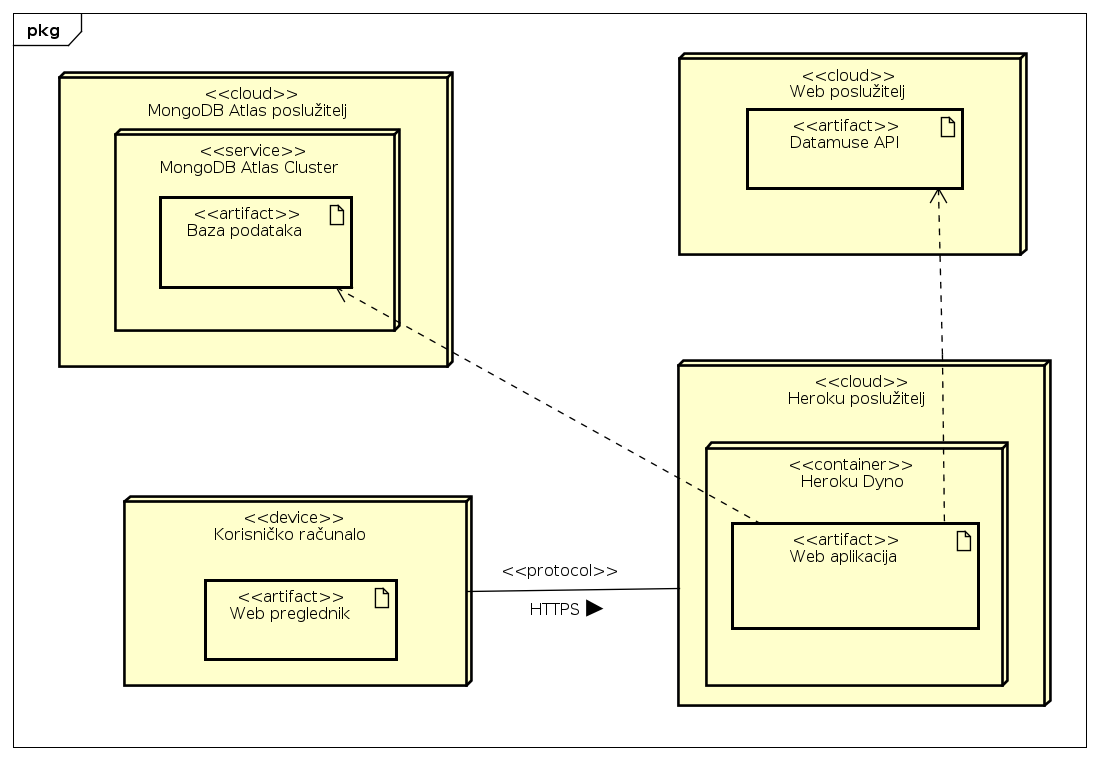
\includegraphics[width=\textwidth]{dijagrami/dijagram_razmjestaja.png} %veličina u odnosu na širinu linije
				\caption{Dijagram razmještaja}
				\label{fig:Dijagram_razmjestaja} %label mora biti drugaciji za svaku sliku
			\end{figure}
			
			\eject 
		
		\section{Upute za puštanje u pogon}
			
			\noindent{\textbf{Konfiguracija poslužitelja baze podataka}}\\
			
			\noindent{\textbf{Konfiguracija baze podataka}}\\
			
			\noindent{\textbf{Konfiguracija Heroku poslužitelja}}\\
			\noindent{Nakon što se uspješno izradi Heroku korisnički račun, potrebno je stvoriti novu aplikaciju u "Dashboardu" klikom na "Create new app". Potrebno je upisati ime aplikacije, odabrati regiju i završiti stvaranje aplikacije klikom na "Create app". Forma za izradu aplikacije je prikazana na slici \ref{fig:StvaranjeAplikacije}}.
			
			
			\begin{figure}[H]
				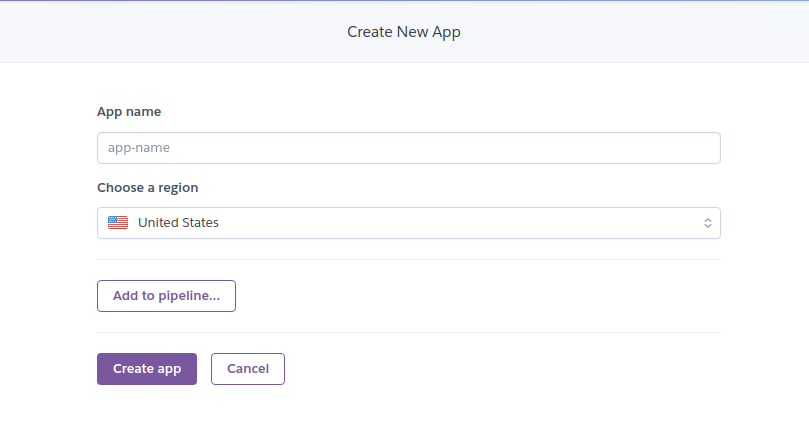
\includegraphics[width=\textwidth]{slike/stvaranjeAplikacije.png} %veličina u odnosu na širinu linije
				\caption{Stvaranje nove aplikacije}
				\label{fig:StvaranjeAplikacije} %label mora biti drugaciji za svaku sliku
			\end{figure}
		
			
			\indent{Nakon izrade aplikacije potrebno je podesiti konfiguraciju u "Settings" dijelu aplikacije kao što je prikazano na slikama \ref{fig:podesi1} i \ref{fig:podesi2}. "DB CONNECTION STRING" se dobije prilikom konfiguracije baze podataka i služi aplikaciji za pristup bazi podataka, a "SECRET KEY" je tajni ključ čija će vrijednost ovisiti o konkretnom projektu, Django ga interno koristi za potrebe hashiranja. Moguće je i podesiti ostale parametre po potrebi.}\\
			\indent{Potrebno je i dodati "Buildpack" za Node.js i Python s obzirom da aplikacija koristi programski jezik Python za backend, a React za frontend. "Buildpackovi" služe za instaliranje svega onoga što je potrebno da bi se aplikacija mogla pokrenuti na Heroku poslužitelju.}
			
			
			\begin{figure}[H]
				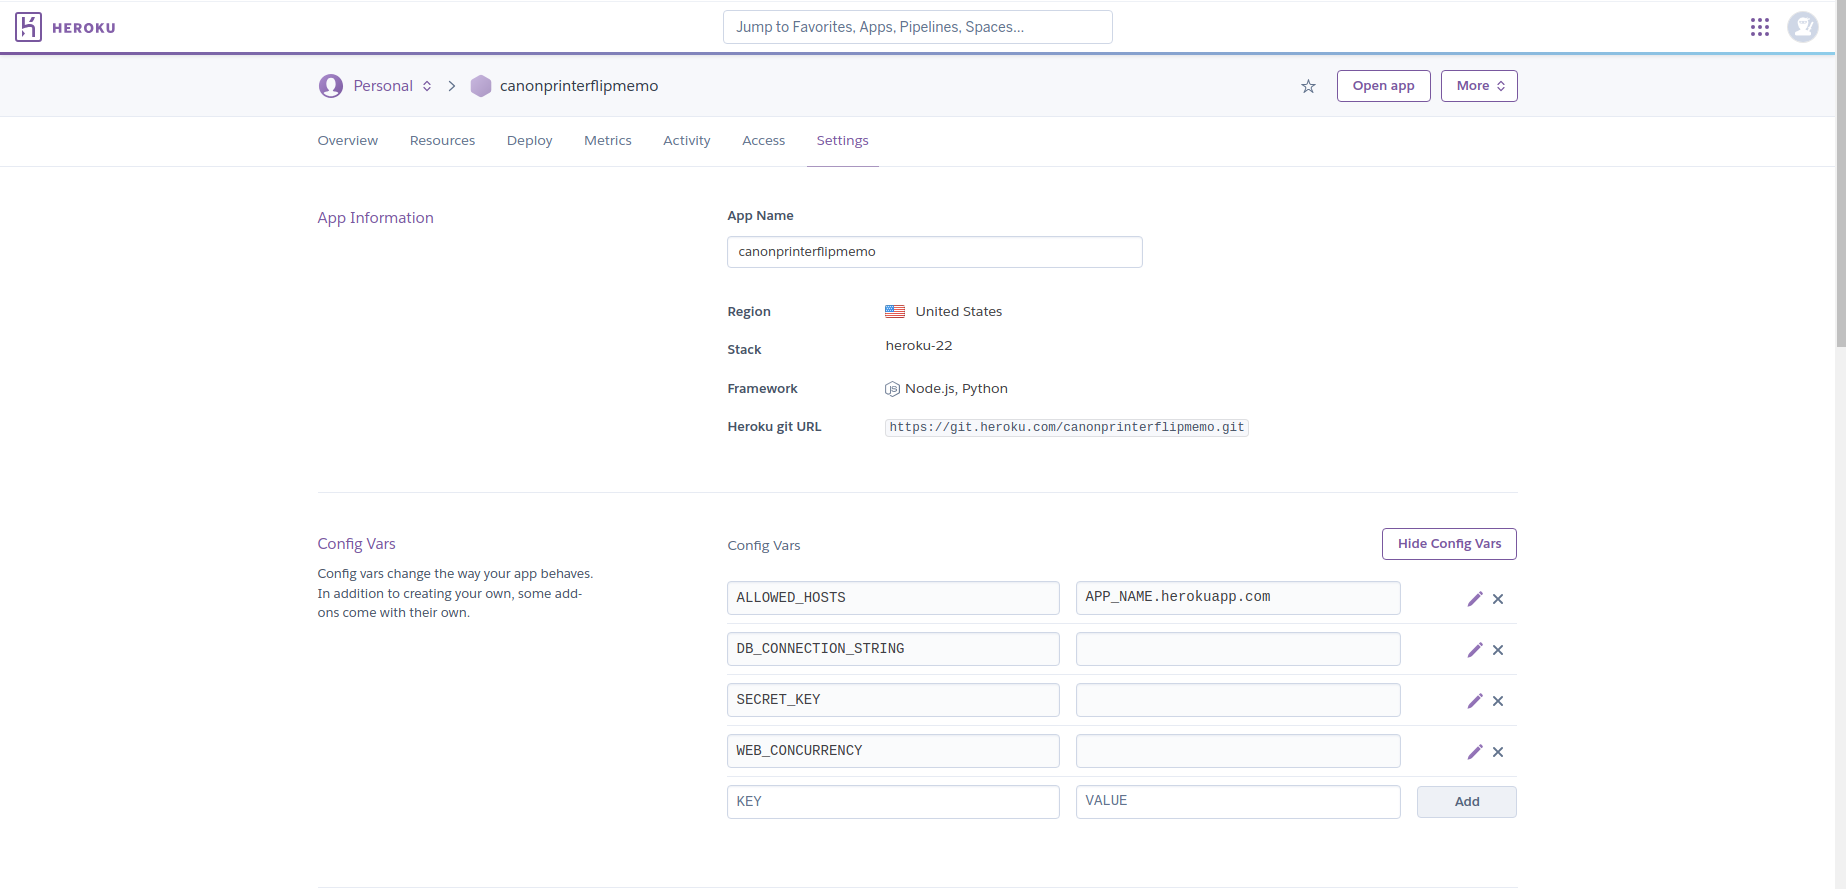
\includegraphics[width=\textwidth]{slike/podesi1.png} %veličina u odnosu na širinu linije
				\caption{Konfiguracija konfiguracijski varijabli}
				\label{fig:podesi1} %label mora biti drugaciji za svaku sliku
			\end{figure}
		
			\begin{figure}[H]
				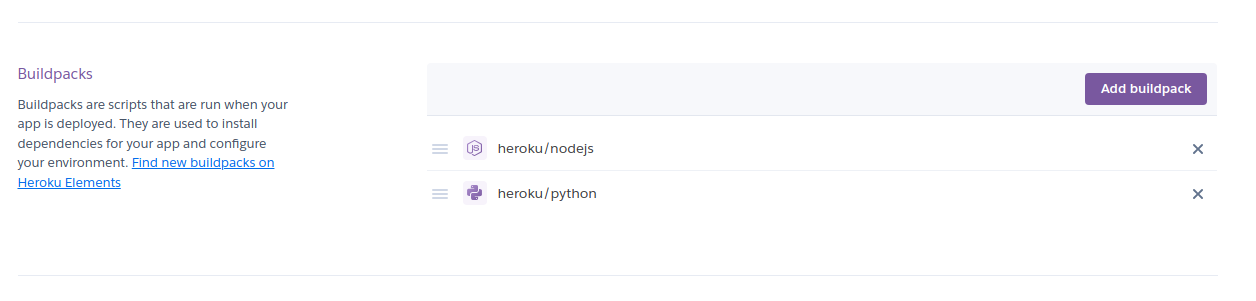
\includegraphics[width=\textwidth]{slike/podesi2.png} %veličina u odnosu na širinu linije
				\caption{Konfiguracija "Buildpackova"}
				\label{fig:podesi2} %label mora biti drugaciji za svaku sliku
			\end{figure}
		
			\noindent{\textbf{Organizacija strukture projekta za puštanje u pogon}}\\
			\noindent{Za potrebe puštanje aplikacije u pogon pomoću Heroku usluge, potrebno je organizirati strukturu projekta odnosno izvornog koda u onakvu strukturu kakvu Heroku očekuje prilikom prijenosa izvornog koda na Heroku poslužitelj. Reorganizacija strukture projekta većim dijelom uključuje reorganizaciju postojeće hijerarhije direktorija, no potrebno je dodati i neke konfiguracijske datoteke što je opisano u nastavku.}\\
			\indent{Na slici \ref{fig:organizacijaKoda} je prikazan primjer strukture projekta kakvu očekuje Heroku. "FlipMemo", "main" i "users" su mape iz Django dijela aplikacije, a "src", "public" iz React dijela aplikacije. Bitno je da sve te mape budu na istoj razini u glavnom direktoriju "CanonPrinter". "staticfiles" mapa je trenutno prazna, no u nju se prilikom puštanja u pogon spremaju razne datoteke nakon što se odradi "build" na Heroku poslužitelju.}
			
			\begin{figure}[H]
				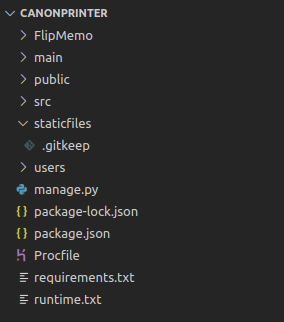
\includegraphics[width=\textwidth]{slike/organizacijaKoda.png} %veličina u odnosu na širinu linije
				\caption{Struktura projekta za puštanje aplikacije u pogon}
				\label{fig:organizacijaKoda} %label mora biti drugaciji za svaku sliku
			\end{figure}
		
			\noindent{"manage.py", "package.json" i "package-lock.json" su datoteke koje postoje i prije reorganizacije strukture projekta, a vezanu su uz Django i React dok su "Procfile", "requirements.txt" i "runtime.txt" konfiguracijske datoteke koje Heroku očekuje da postoje u projektu i moraju se dodati prije puštanja aplikacije u pogon. Sadržaj konfiguracijskih datoteke prikazan je na slikama \ref{fig:konf1}, \ref{fig:konf2}, \ref{fig:konf3}. 
			
			\begin{figure}[H]
				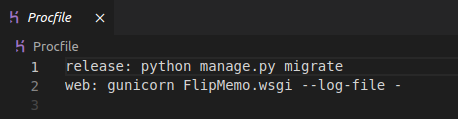
\includegraphics[width=\textwidth]{slike/konf1.png} %veličina u odnosu na širinu linije
				\caption{Procfile}
				\label{fig:konf1} %label mora biti drugaciji za svaku sliku
			\end{figure}
		
			\begin{figure}[H]
				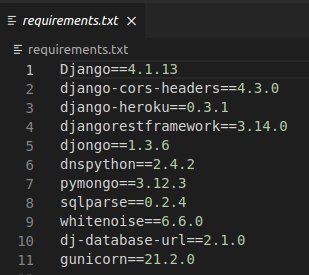
\includegraphics[width=\textwidth]{slike/konf2.png} 	%veličina u odnosu na širinu linije
				\caption{requirements.txt}
				\label{fig:konf2} %label mora biti drugaciji za svaku sliku
			\end{figure}
		
			Svaka konfiguracijska datoteka sadrži konfiguracijske parametre koji su potrebni prilikom puštanja aplikacije u pogon, npr. verzije svih potrebnih biblioteka koje je potrebno instalirati, verziju programskog jezika Python i sl. Za detalje o tome kako Heroku koristi te konfiguracijske datoteke upućujemo na službenu dokumentaciju\footnote{\url{https://devcenter.heroku.com/categories/reference}}.}
	
			\begin{figure}[H]
				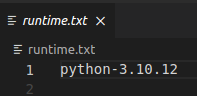
\includegraphics[width=\textwidth]{slike/konf3.png} %veličina u odnosu na širinu linije
				\caption{runtime.txt}
				\label{fig:konf3} %label mora biti drugaciji za svaku sliku
			\end{figure}
		
			\noindent{\textbf{Puštanje aplikacije u pogon korištenjem Heroku Git}}\\
			\noindent{Nakon provedenih svih potrebnih prethodno opisanih koraka, aplikacije se može pustiti u pogon na Heroku poslužitelj na više načina. Ovdje prikazujemo način puštanja aplikacije u pogon korištenjem Heroku Gita. Potrebno je instalirati Heroku CLI koji omogućuje rad sa Heroku korištenjem komandne linije \footnote{\url{https://devcenter.heroku.com/articles/heroku-cli}}.}\\
			\indent{Nakon što je Heroku CLI uspješno instaliran za odgovarajuću platformu, potrebno je provesti postupak prijenosa izvornog koda projekta na Heroku poslužitelj kojim se automatski pokreće i proces izgradnje i puštanja aplikacije u pogon. Slika \ref{fig:herokucli} prikazuje sve potrebne korake kod rada sa Heroku CLI. Aplikacija je nakon provedenih koraka dostupna na poveznici koju je izgenerirao proces puštanja aplikacije u pogon. Moguće je i zadati svoju vlastitu domenu na kojoj će aplikacija biti dostupna što je prikazano na slici \ref{fig:customDomena}}.
			
			\begin{figure}[H]
				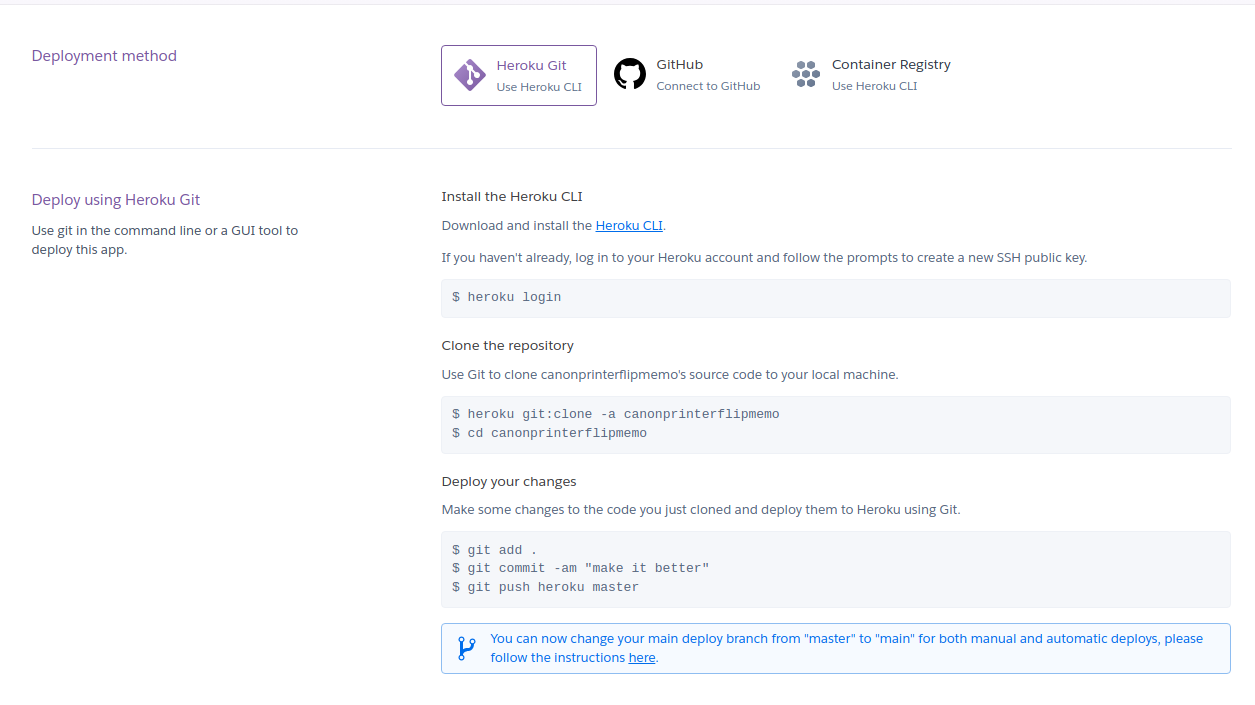
\includegraphics[width=\textwidth]{slike/herokucli.png} %veličina u odnosu na širinu linije
				\caption{Puštanje aplikacije u u pogon korištenjem Heroku CLI}
				\label{fig:herokucli} %label mora biti drugaciji za svaku sliku
			\end{figure}
		
			\begin{figure}[H]
				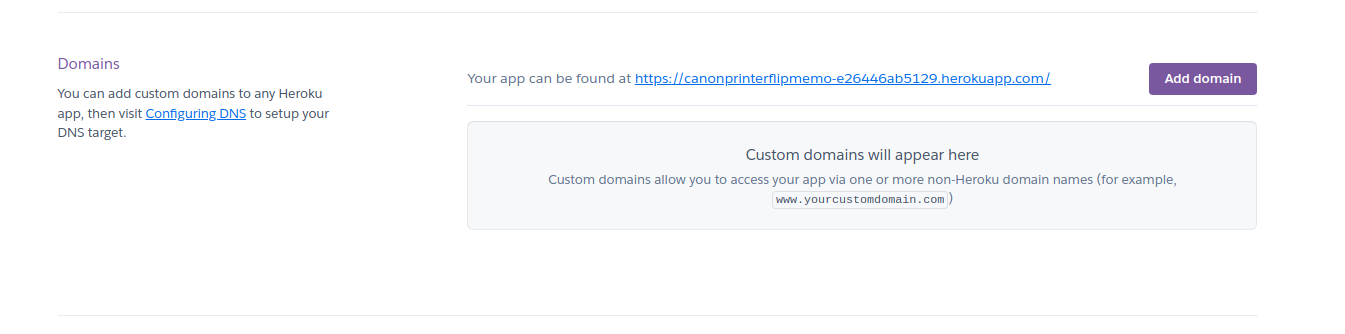
\includegraphics[width=\textwidth]{slike/customDomena.png} %veličina u odnosu na širinu linije
				\caption{Dio postavka za podešavanje domene aplikacije}
				\label{fig:customDomena} %label mora biti drugaciji za svaku sliku
			\end{figure}
			
			\eject 